\section{Introduction}\label{sec:intro}

A broad goal of machine learning is to develop unified architectures 
capable of learning and reasoning over a wide range of tasks and data modalities, such as text, audio, time-series, and images. The generality of the input and output formats for sequence models such as Transformers makes them promising candidates for this goal. However,
a tension exists between the goal of a having a general architecture and 
the ability to support inductive biases that may be favorable for certain types of 
tasks. Recent research has shown that the 
standard Transformer architecture lacks the ability to efficiently
represent relational information, leading to several proposals 
for alternative architectures to encode inductive biases for relational learning 
\citep{santoroRelationalRecurrentNeural2018,shanahanExplicitlyRelationalNeurala,webbEmergentSymbolsBinding2021,kergNeuralArchitectureInductive2022,altabaaLearningHierarchicalRelational2024a,altabaaAbstractorsRelationalCrossattention2023a,webbRelationalBottleneckInductive2024}. Relational architectures, on the other hand, 
fail to provide the generality required to handle more general learning tasks.
In this paper we present an extension of the Transformer architecture that preserves 
the generality of the architecture while allowing for inductive biases to capture the relations between objects. 

General purpose learning architectures can often be understood from the perspective of routing information using message-passing operations, 
where an information retrieval operation is followed by local information processing.
To process a sequence $x_1,\ldots, x_n$ of $n$ objects, this takes the form
\begin{equation}\label{eq:intro_message_passing}
  \begin{split}
    x_i &\gets \mathrm{Aggregate}\bigparen{x_i, \set{m_{j \to i}}_{j=1}^{n}} \\
    x_i &\gets \mathrm{Process}(x_i)
  \end{split}
\end{equation}
Two distinct types of information need to be encoded in the messages $m_{j \to i}$ that
are transmitted from sender $j$ to receiver $i$. The first we refer to 
as \textit{sensory information}, which includes attributes or features 
particular to a specific object.  The second is \textit{relational information} 
about the relationship between the sender and receiver along various dimensions. 
In the case of Transformers, the self-attention mechanism can be
seen as sending messages from object $j$ to object $i$ that are encodings of the sender's features, with $m_{j \to i} = \phi_v(x_j)$. These messages 
are then aggregated according some selection criterion based on the receiver's features,  typically given by the softmax attention scores. The crucial point is that in the Transformer architecture, no explicit representation of the \textit{relation} between the sender and the receiver in encoded in the messages.

In this work, we propose a novel type of attention head that explicitly encodes learned  relations between the sender and receiver. For this type of attention head, the message from the sender object to the receiver object is a set of relations between them, which can be expressed as $m_{j \to i} = r(x_i, x_j)$, with the relations $r(\cdot,\cdot)$ computed through inner products. By combining this with the standard attention mechanism of Transformers, we obtain a model that explicitly processes both sensory and relational information by stacking the two types of attention heads with $m_{j \to i} = (\phi_v(x_j), r(x_i, x_j))$. The proposed architecture is a natural fusion of the Transformer and Abstractor archictectures, which was recently developed to model relational 
learning in a manner that enforces a relational bottleneck 
\citep{altabaaAbstractorsRelationalCrossattention2023a,webbRelationalBottleneckInductive2024}. By combining relational and sensory attention 
heads, this \textit{Dual Attention} architecture disentangles the two types of information in the aggregation phase of attention, while making both types of information available during the information processing stage. 

\jlnote{More about Abstractors here, how we're building on it?}

A series of four experiments across a range of data types demonstrates how the Dual Attention Transformer architecture preserves the benefits of standard Transformers while leading to greater efficiency of learning by combining relational information and sensory information. To begin, we use the Relational Games dataset which tests
a model's ability to identify a particular visual relationship among a series of objects. We use a type of Vision Transformer architecture~\citep{dosovitskiyImageWorth16x162020}, 
and evaluate learning curves of the models, finding that the Dual Attention architecture 
is significantly more sample efficent compared to a standard Transformer. 
Next, we evaluate the Dual Attention architecture on a set of mathematical problem-solving tasks based on the benchmark contributed by~\citet{saxtonAnalyzingMathematicalReasoning2019}, where the tasks range from 
to differentiating functions, finding that the Dual Attention models learn faster and reach higher accuracies compared to a standard Transformer. 
We also evaluate the new architecture on autoregressive language modeling.
Using the Tiny Stories dataset of~\citet{eldanTinyStoriesHowSmall2023} to train models on the roughly the scale of GPT-2, 
we fix the total number of attention heads, and compare a Transformer with only standard self-attention heads to Dual Attention models with a mix of self-attention and relational attention heads, finding that the Dual Attention models achieve a smaller validation loss for the same total number of attention heads. Finally, 
we again use a Vision Transformer for classification of ImageNet images \citep{dosovitskiyImageWorth16x162020}, and find improved efficiency 
of learning. This suggests that relational processing is important in processing visual scenes, matching the intuition that parsing a visual scene requires reasoning about the visual relations between different objects or parts of the scene. Together, the experiments 
show that the Dual Attention Transformer is effective across a range of tasks and data types.


%\begin{enumerate}
%\item Summarize key ideas and basic elements of our proposed architecture
%  \item Summarize our experimental results and what they indicate
%  \item Summarize technical contributions in clear concise bullets
%\end{enumerate}

\aanote{TODO: add discussion of some related work. perhaps as separate related work section? explain why it's so important to explicitly represent relational features (perhaps give some examples)}

The contributions in this paper are summarized as follows:
\begin{enumerate}
  \item We introduce a new Relation Attention mechanism that disentangles sensory information from relational information. While the standard self-attention mechanism uses relations to define the attention weights, Relational Attention uses learned relations in the values that are transmitted during message passing. 
  \item We introduce a generalized Transformer architecture that uses Dual Attention, so that heads can either encode sensory or relational information. The Relational Attention heads can use several different mechanisms to assign abstract symbols as values, combined with the learned relations. 
  \item We carry out an extensive set of experiments across different tasks and data modalities, showing that the Dual Attention Transformer outperforms standard Transformers in terms of data efficiency. Moreover, the new architecture can be used wherever a Transformer is used, with little loss in computational efficiency.
\end{enumerate}

Note that throughout the paper, the term ``sensory'' is used as shorthand to refer to the features and attributes of an individual object. For example, in a language task, this could be the components of a word embedding, and in a vision task, this could be 
the pixel values of a patch of an image or the feature maps obtained using a CNN. We use the term ``relational'' to refer to information about the relationship between the features of two objects. For example, in a language task, this could be the grammatical, syntactic, or semantic relation between two words. In a vision task, this could be a representation of similarity across different visual attributes such as the color, texture 
or semantic category of two objects. In the proposed learning architecture, 
the sensory information and relations are both learned, rather than being specified in advance of processing data for a given task.  The generic term ``object'' 
is used to refer to elements of the input, which is typically a sequence or set. 
For example, objects might be the tokens in the context of text or the patches of an image in the context of vision.

\begin{figure}[t]
  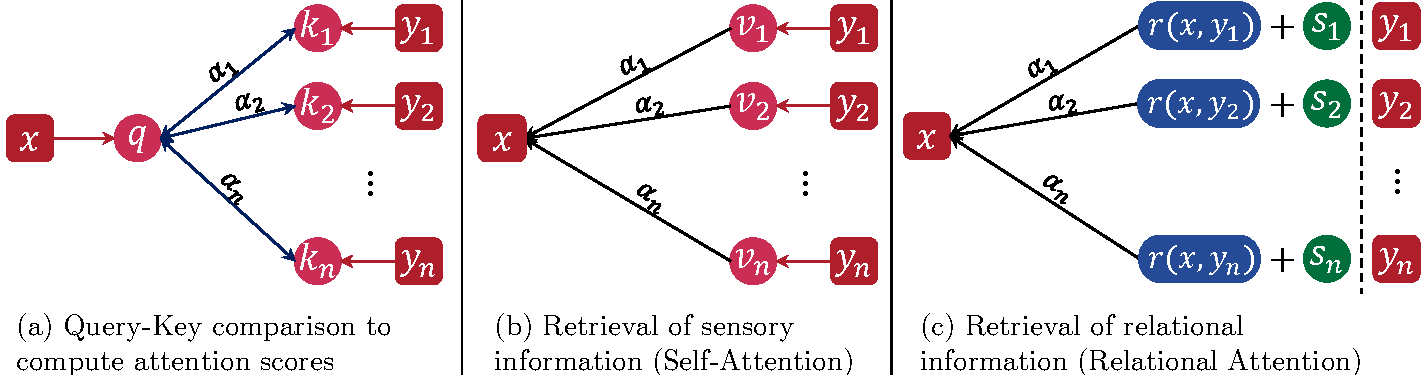
\includegraphics[width=\textwidth]{figs/attn_fig_combined.pdf}
  \caption{A depiction of $\Attn(x, \ys)$ and $\RelAttn(x, \ys)$. Both forms start with a query-key comparison to select objects to attend to. Self-attention retrieves sensory information about the attributes of individual objects while relational attention retrieves relational information about the relationship between the attended objects and the receiver.}\label{fig:selfattn_relattn}
\end{figure}
